\section{Results}
\label{sec:results}

\subsection{Fault detection on \sheetfault}
\label{sec:e1}
\begin{table*}[!t]
\caption{Fault detection on \textsc{SheetFault} (13{,}356 faulty and 10{,}892 clean formulas, micro-averaged, \%). \emph{Reject} counts a formula as detected only if it is blocked; \emph{flag} also counts warnings. FPR is the share of clean formulas that is rejected or flagged.}
\label{tab:e1-overall}

\centering\footnotesize
\begin{tabular}{l rrrr rrrr}
\toprule
& \multicolumn{4}{c}{\textbf{Reject policy} (block on error)} & \multicolumn{4}{c}{\textbf{Flag policy} (error or warning)} \\
\cmidrule(lr){2-5}\cmidrule(lr){6-9}
\textbf{Detector} & P & R & F1 & FPR & P & R & F1 & FPR \\
\midrule
Accept all & -- & 0.0 & -- & 0.0 & -- & 0.0 & -- & 0.0 \\
Syntax only & 100.0 & 17.6 & 29.9 & 0.0 & 100.0 & 17.6 & 29.9 & 0.0 \\
Linter & 96.2 & 27.2 & 42.4 & 1.3 & 96.2 & 27.2 & 42.4 & 1.3 \\
Shipped (v1) & 100.0 & 44.2 & 61.3 & 0.0 & 85.2 & 69.2 & 76.4 & 14.7 \\
GroundCheck & \textbf{100.0} & \textbf{83.0} & \textbf{90.7} & 0.0 & \textbf{98.8} & \textbf{92.4} & \textbf{95.5} & 1.3 \\
\bottomrule
\end{tabular}
\end{table*}


A lexical check blocks only \eonesyntaxrejectR\% of faults and a function linter \eonelintrejectR\% (Table~\ref{tab:e1-overall}): most benchmark faults are well formed and name things that do not exist or do not fit the data. The shipped verifier blocks \eonevonerejectR\% (F1 \eonevonerejectF) with no false positives, but \eonevoneflagR\% only if warnings count, and then \eonevoneflagFPR\% of clean formulas are flagged: its row-bounds warning fires on every formula with headroom (\cleanHeadroomVone\% of those) and its function list omits common functions such as \code{AVERAGEIF} and \code{MAXIFS}, so \cleanGoldVone\% of the \emph{gold} formulas are flagged. \gc{} blocks \eonevtworejectR\% (F1 \eonevtworejectF) at \eonevtworejectFPR\% false positives; counting warnings, recall is \eonevtwoflagR\% at FPR \eonevtwoflagFPR\%, and every flagged clean formula is a custom function missing from the official list (a warning by design; Table~\ref{tab:e1-clean}, Appendix~\ref{app:bench}, gives the false-alarm rate for every clean class).

The headline difference is large and does not depend on how uncertainty is counted. Resampling the \clWbN{} workbooks rather than the formulas gives a 95\% interval of [\clVtwoRecallLo, \clVtwoRecallHi]\% for the recall of \gc{} and [\clVoneRecallLo, \clVoneRecallHi]\% for the shipped verifier, a paired difference of \clDiffRecall{} points [\clDiffRecallLo, \clDiffRecallHi], and \gc{} is ahead in \clWbBetter{} of \clWbN{} workbooks. These intervals are narrow because one generator produces every workbook, so they measure sampling noise, not how representative the benchmark is. The benchmark was written with the verifier; Section~\ref{sec:e1b} tests it on real formulas.

Figure~\ref{fig:e1-classes} and Table~\ref{tab:e1-classes} (Appendix~\ref{app:results}) show where the gain comes from. The shipped verifier cannot see a range that contains its own cell (\clsrangecontainsselfvoneReject\% blocked), a whole-column self-inclusion (\clscolumncontainsselfvoneReject\%), a cycle through a range (\clscycleindirectrangevoneReject\%), a header used as a name (\clsheaderasnamevoneReject\%), unequal range sizes (\clsrangesizemismatchvoneReject\%) or an out-of-range lookup index (\clslookupindexoobvoneReject\%): its graph links a range to one node, never to the formula cells inside it, so the totals-row mistake is invisible. \gc{} blocks all of them. Hallucinated function names are blocked only as near-misses (\clsghostfunctionvtwoReject\%) and otherwise warned about (\clsghostfunctionvtwoFlag\% flagged), as intended for a language with custom functions; an absent criterion and an aggregate over text are flagged (\clsghostvaluevtwoFlag\% and \clstypemismatchvtwoFlag\%) but never rejected; the two semantic classes (\clswrongnumericcolN{} and \clswrongfunctionN{} instances) are essentially undetectable, as they must be.

\begin{figure}[t]
\centering
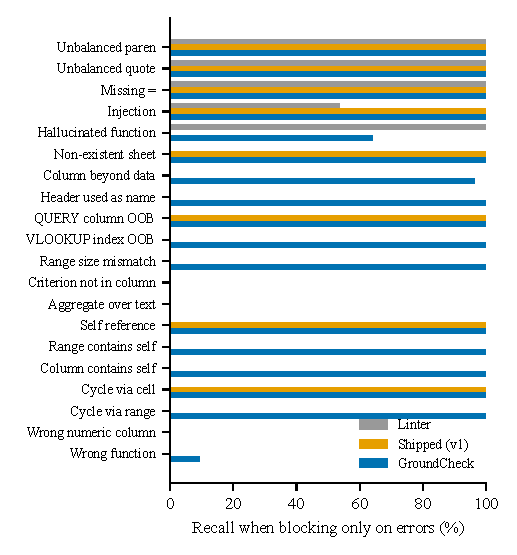
\includegraphics[width=0.95\columnwidth]{figures/fig_e1_classes}
\caption{Recall per fault class when a formula is blocked only on errors.}
\label{fig:e1-classes}
\end{figure}

\begin{table}
\caption{Leave-one-layer-out ablation of the verifier on \textsc{SheetFault} (\%).}
\label{tab:e1-ablation}

\centering\footnotesize
\begin{adjustbox}{max width=\columnwidth}\begin{tabular}{l rr rr}
\toprule
& \multicolumn{2}{c}{\textbf{Reject}} & \multicolumn{2}{c}{\textbf{Flag}} \\
\cmidrule(lr){2-3}\cmidrule(lr){4-5}
\textbf{Configuration} & R & F1 & R & F1 \\
\midrule
All layers & 83.0 & 90.7 & 92.4 & 95.5 \\
$-$ structural + parse & 62.4 & 76.9 & 71.9 & 83.1 \\
$-$ symbols & 66.5 & 79.9 & 73.6 & 84.8 \\
$-$ bounds & 78.5 & 87.9 & 87.9 & 93.0 \\
$-$ shape & 79.2 & 88.4 & 88.6 & 93.4 \\
$-$ grounding & 83.0 & 90.7 & 85.3 & 91.5 \\
$-$ circularity & 50.6 & 67.2 & 66.5 & 79.4 \\
$-$ QUERY columns & 81.9 & 90.1 & 91.3 & 94.9 \\
\bottomrule
\end{tabular}\end{adjustbox}
\end{table}


Removing one layer at a time (Table~\ref{tab:e1-ablation}), circularity matters most (reject recall \eonevtworejectR\% $\to$ \ablcircularRejectR\%), then the parse (\ablstructuralRejectR\%) and symbols (\ablsymbolsRejectR\%). Grounding leaves reject recall unchanged because its findings are warnings. Of the \visloudN{} loud faults \gc{} blocks \visloudvtwoReject\% (shipped: \visloudvoneReject\%); of the \vissilentN{} silent faults, which would write a plausible wrong value into the sheet, it blocks \vissilentvtwoReject\% and flags \vissilentvtwoFlag\% (shipped: \vissilentvoneReject\% and \vissilentvoneFlag\%; Figure~\ref{fig:e1-visibility}). The rest are the semantic swaps: verification turns most silent failures into visible ones but does not make an agent correct.

\begin{figure}[t]
\centering
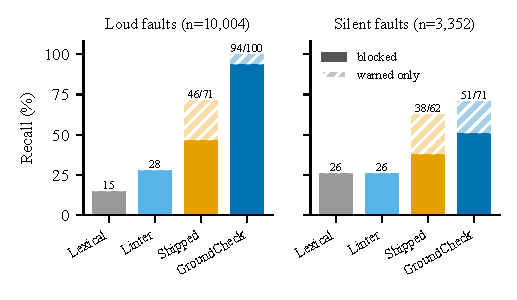
\includegraphics[width=\columnwidth]{figures/fig_e1_visibility}
\caption{Recall on loud and silent faults. Solid: the formula is blocked; hatched: only a warning is raised.}
\label{fig:e1-visibility}
\end{figure}

The result does not depend on the workbook domain (Figure~\ref{fig:e1-domain}): reject recall is \domVtwoMin--\domVtwoMax\% for \gc{} and \domVoneMin--\domVoneMax\% for the shipped verifier in each of the six domains, with \domVtwoFPRMax\% false positives in every one; across the \domWbN{} individual workbooks it ranges from \domWbMin\% to \domWbMax\% (shipped: \domWbVoneMin--\domWbVoneMax\%), so no single workbook accounts for the gain.

\begin{figure}[t]
\centering
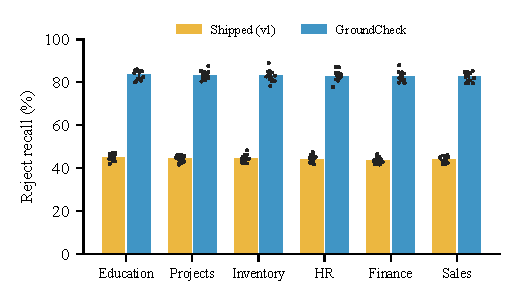
\includegraphics[width=\columnwidth]{figures/fig_e1_domain}
\caption{Reject recall by workbook domain, with 95\% Wilson intervals; each dot is one of the 12 workbooks of the domain.}
\label{fig:e1-domain}
\end{figure}

\subsection{Real-world formulas}
\label{sec:e1b}
\paragraph{Development and held-out sets}
On the development set the first runs exposed two defects in our verifier, a tokenizer gap for row ranges with absolute markers (\code{\$1:\$1}) and a circularity false positive on \code{ROWS(B\$2:B83)} placed in B83, and one in our corpus extraction (Excel defined names were not loaded). After fixing them the development rejection rate is \rwDevvtwoReject\% (shipped verifier: \rwDevvoneReject\%). The held-out set, scored once, gives \rwcTVoneReject\% for the shipped verifier and \rwcTVtwoReject\% for \gc{} on \rwcTFormulas{} formulas from \rwcTWorkbooks{} workbooks (flag policy: \rwvoneFlag\% and \rwvtwoFlag\%). After seeing it we exempted \code{COUNTA}, \code{COUNTBLANK} and \code{ISBLANK} when they point at empty cells, which lowers the rate to \rwvtwoRejectPost\%; the first-pass figure is the held-out result, because the second was tuned on this set.

By rejection rate the two verifiers are not distinguishable: the difference is \rwcTDiff{} points (workbook-clustered 95\% interval [\rwcTDiffLo, \rwcTDiffHi]; Table~\ref{tab:rw-sets}). Rejections are concentrated. Only \rwcTWbRejected{} of the 300 workbooks contain a rejection of a real formula, and the five workbooks with the most rejections hold \rwcTTopfiveShare\% of them, which is why these intervals are far wider than formula-level ones.

\begin{table}
\caption{Share of real-world formulas (\%) rejected, with 95\% intervals from a bootstrap over workbooks (300 workbooks per set). Rejections are concentrated in a few workbooks, so these intervals are much wider than formula-level ones.}
\label{tab:rw-sets}

\centering\footnotesize
\begin{adjustbox}{max width=\columnwidth}\begin{tabular}{l r c c}
\toprule
\textbf{Set} & \textbf{Formulas} & \textbf{Shipped} & \textbf{\gc} \\
\midrule
Held-out, before the change & 5{,}184 & 8.8 [5.8, 12.1] & 8.6 [5.6, 11.8] \\
Confirmation 1, frozen v2 & 5{,}537 & 9.0 [5.6, 12.3] & 10.4 [6.8, 13.9] \\
Confirmation 2, frozen v2.1 & 5{,}277 & 6.4 [3.9, 9.2] & 7.6 [4.8, 10.5] \\
\bottomrule
\end{tabular}\end{adjustbox}
\end{table}


\begin{figure}[t]
\centering
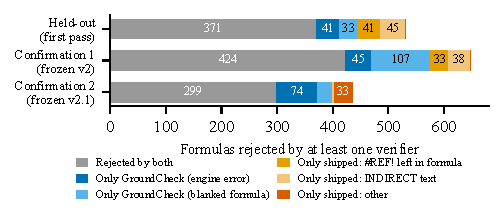
\includegraphics[width=\columnwidth]{figures/fig_rw_overlap}
\caption{Where the two verifiers disagree on real formulas: the formulas rejected by at least one of them, by who rejects them. Formulas blanked by the dataset's PII pass count as artifacts. Confirmation set~2 was scored with the extended verifier.}
\label{fig:rw-overlap}
\end{figure}

\paragraph{Confirmation set, verifier frozen}
The confirmation set (\rwcFFormulas{} formulas from \rwcFWorkbooks{} workbooks), scored once with the frozen verifier, gives \rwcFVoneReject\% for the shipped verifier and \rwcFVtwoReject\% for \gc{}, a difference of \rwcFDiff{} points [\rwcFDiffLo, \rwcFDiffHi]. Of the \rwcFRejected{} rejections by \gc, \rwcFEmpty{} are formulas that the dataset's PII pass blanked to \code{=}; they are not real formulas, and without them the rate is \rwcFVtwoRejectNoEmpty\% [\rwcFVtwoRejectNoEmptyLo, \rwcFVtwoRejectNoEmptyHi]. For \rwcFEngineConfirmedReal{} of the other \rwcFRealRejected{} the independent engine also returns an error (Appendix~\ref{app:results}). Most of the rest reference sheets that do not exist, \rwcFGhostOkMasked{} of them inside \code{IFERROR} or a similar wrapper: the formula is broken and the wrapper hides it, a latent fault that no check on values can see.

The sets show where the two verifiers differ (Figure~\ref{fig:rw-overlap}). Both reject \rwcFOBoth{} formulas. Only \gc{} rejects \rwcFOOnlyVtwoReal{} real formulas (the engine returns an error for \rwcFOOnlyVtwoEngineError{} of them), chiefly circular references and ranges beyond the data. Only the shipped verifier rejects \rwcFOOnlyVone{}. \rwcFOOnlyVoneRefLiteral{} of them contain a literal \code{\#REF!}, a reference deleted from the formula, which the shipped verifier catches by accident because it reads \code{REF!} as a sheet name; \rwcFOOnlyVoneIndirect{} are \code{INDIRECT} calls whose text names a sheet that does not exist, or builds the name by concatenation; these are \gc's misses. The remaining \rwcFOOnlyVoneOther{} is a parsing error of the shipped verifier on a sheet name that contains a quote. Neither class is in \sheetfault, and \gc{} checked neither: a benchmark written with the verifier cannot show a gap that the authors' idea of faults did not include. The held-out set held the same gap (\rwcTORefLiteralInAnyFormula{} formulas with \code{\#REF!}), which we had not examined from this angle. Deleted references are not rare: \rwcFORefLiteralInAnyFormula{} of \rwcFFormulas{} confirmation formulas contain one.

\ifdefined\rwcGFormulas
\paragraph{Closing the gap, and a second confirmation}
We extended \gc{} by two rules: a literal \code{\#REF!} or \code{\#NAME?} in a formula is an error, and an \code{INDIRECT} whose text starts with a sheet name is checked against the workbook's sheets. The rules change none of the \eqInstances{} \sheetfault{} verdicts (\eqDiff{} differ) and can fire on none of the \eqFormulas{} formulas the models generated (\eqHits{} do), so the benchmark and end-to-end results hold for the extended verifier. Scored again on the real formulas, the extended verifier rejects \rwcTPVtwoReject\% of the held-out and \rwcFPVtwoReject\% of the confirmation formulas, but these figures are post hoc, since both sets informed the rules. The confirmatory test is a second confirmation set (\rwcGFormulas{} formulas from \rwcGWorkbooks{} workbooks, from a later part of the archive), scored once with the extended verifier frozen: the shipped verifier rejects \rwcGVoneReject\% and \gc{} \rwcGVtwoReject\% (difference \rwcGDiff{} points [\rwcGDiffLo, \rwcGDiffHi]; without blanked formulas \rwcGVtwoRejectNoEmpty\%). Of the \rwcGOOnlyVone{} formulas that only the shipped verifier rejects, \rwcGOOnlyVoneRefLiteral{} contain \code{\#REF!}; reading all of them, the rest are spurious rejections: it takes parentheses and \code{!} inside text literals for code, and treats an \code{INDIRECT} whose sheet name comes from a named range as a missing sheet (the engine evaluates \rwcGOOnlyVoneEngineOk{} of them without error). The \rwcGOOnlyVtwoReal{} real formulas that only \gc{} rejects all produce an engine error (\rwcGOOnlyVtwoEngineError{}).
\fi

Taken together, between about 6\% and 11\% of real formulas are rejected by either verifier, the rejections sit in a few workbooks, and \gc{} rejects one to two points more than the shipped verifier, a difference whose workbook-clustered interval includes zero in every set. The larger gain that \sheetfault{} shows does not appear in the rejection rate on real formulas. What differs is the kind of rejection. Where the verifiers disagree, the formulas that only \gc{} rejects are engine-confirmed errors (\rwcFOOnlyVtwoEngineError{} of \rwcFOOnlyVtwoReal{} in confirmation set~1\ifdefined\rwcGFormulas, \rwcGOOnlyVtwoEngineError{} of \rwcGOOnlyVtwoReal{} in set~2\fi)\ifdefined\rwcGFormulas, and, once deleted references are covered, the \rwcGOOnlyVone{} formulas that only the shipped verifier rejects in set~2 are all spurious\fi. This is supporting evidence, not a precision figure, since it rests on one engine and on our reading of the formulas. The benchmark measures coverage of the fault classes we designed; real formulas contain some of them rarely and others, such as deleted references, that we had not listed.

\subsection{End-to-end accuracy with real models}
\label{sec:e5}
We run the production formula agent with two local models, \efAName{} and \efBName, and three hosted ones, \efDName, \efEName{} and \efFName{} (Section~\ref{sec:e5method}). With the final system the first attempt is correct for \efAfinal\% of the \efAN{} tasks with \efAName{} and \efBfinal\% with \efBName; the hosted models reach \efDfinal\% (\efDN{} tasks), \efEfinal\% (\efEN) and \efFfinal\% (\efFN).

\paragraph{Retrieved context needs column letters}
\begin{table}
\caption{Attempt-1 execution accuracy (\%) by context. Lookup tasks read a sheet other than the active one; ``Other'' tasks read the active sheet only. The only difference between the two retrieved rows is that table chunks now carry column letters and the data-row span.}
\label{tab:e5-context}

\centering\footnotesize
\begin{adjustbox}{max width=\columnwidth}\begin{tabular}{l l rrr}
\toprule
\textbf{Model} & \textbf{Context} & \textbf{All} & \textbf{Lookup} & \textbf{Other} \\
\midrule
\multirow{3}{*}{Llama~3.1 8B} & Active sheet only & 72.2 & 3.3 & 78.5 \\
 & Retrieved (shipped) & 64.4 & 0.0 & 70.3 \\
 & Retrieved + letters & \textbf{70.8} & 0.0 & 77.3 \\
\midrule
\multirow{2}{*}{Llama~3.2 3B} & Active sheet only & 37.5 & 3.3 & 40.6 \\
 & Retrieved + letters & \textbf{38.9} & 3.3 & 42.1 \\
\midrule
\multirow{2}{*}{Llama~3.1 8B, new tasks} & Active sheet only & 76.7 & 0.0 & 80.7 \\
 & Retrieved + letters & \textbf{72.2} & 0.0 & 76.0 \\
\midrule
\multirow{2}{*}{Gemini~3.1 Flash-Lite} & Active sheet only & 89.2 & 31.8 & 95.0 \\
 & Retrieved + letters & \textbf{96.7} & 95.5 & 96.8 \\
\midrule
\multirow{2}{*}{Gemini~3.5 Flash-Lite} & Active sheet only & 89.9 & 27.3 & 96.0 \\
 & Retrieved + letters & \textbf{95.2} & 95.5 & 95.1 \\
\midrule
\multirow{2}{*}{Gemma~4 26B-A4B} & Active sheet only & 91.1 & 36.7 & 96.1 \\
 & Retrieved + letters & \textbf{95.8} & 96.7 & 95.8 \\
\bottomrule
\end{tabular}\end{adjustbox}
\end{table}

With the shipped active-sheet context \efAName{} reaches \efAflat\% at attempt 1 (Table~\ref{tab:e5-context}). Adding the ranked context in the chunk format the add-on shipped \emph{lowered} accuracy to \efAshipped\% (\efATestshippedvsflatB{} tasks favour the active sheet alone, \efATestshippedvsflatA{} the retrieved context; $p$ \efATestshippedvsflatP, exact McNemar). Those chunks listed columns by header only, so the model guessed letters (a silently wrong numeric column), wrote headers as names (\code{COUNTIF(Lead Time,">31")}) or invented functions. With each column's letter and the data-row span in the chunk, accuracy is \efAfinal\% ($p$ \efATestfinalvsshippedP{} against the shipped format), indistinguishable from the active sheet alone ($p$ \efATestfinalvsflatP): retrieval does not help on tasks that read the active sheet; its purpose is cross-sheet requests. There the first attempt is correct \efAfinalLookup\% of the time on the \efAfinalLookupN{} lookup tasks, because of the prompt rather than the context: \efALkSheetTwo{} of \efALkN{} attempts copied \code{Sheet2} from the agent's own worked example (Section~\ref{sec:discussion}). For the hosted models the retrieved context is what matters: it raises accuracy from \efDflat\%, \efEflat\% and \efFflat\% with the active sheet alone to \efDfinal\%, \efEfinal\% and \efFfinal\%, almost entirely on cross-sheet lookups (\efDflatLookup\% to \efDfinalLookup\% for \efDName).
\ifdefined\efCN
\emph{Held-out confirmation.} On \efCN{} tasks from fresh workbooks the final chunk format gives \efCfinal\% at attempt 1 against \efCflat\% for the active sheet alone ($p$ \efCTestfinalvsflatP), the same picture as on the main set. \gc{} feedback raises it to \efCSvtwofb\% ($+$\efCSvtwofbD{} points, Holm-adjusted $p$ \hmCHolmVtwoRes{} against resampling) and, with suspicious findings, to \efCSvtwofbplussusp\% ($p$ \hmCHolmSuspRes): the same direction with less power.
\fi

\paragraph{What verification sees}
Of the \efAWrong{} formulas \efAName{} gets wrong at attempt 1, \efALoud{} (\efALoudShare\%) are loud and \efASilent{} are silent (Figure~\ref{fig:e5-taxonomy}; Table~\ref{tab:e5-taxonomy}, Appendix~\ref{app:results}). \gc{} rejects \efACaughtTwo{} of them (the shipped verifier \efACaughtOne{}) and flags \efAFlagTwo{} in all; it rejects none of the silent ones and flags \efASilentFlagTwo{}. None of the \efANCorrect{} correct formulas is rejected. The rejections are concentrated: 29 of the 35 are references to a sheet that does not exist (the \code{Sheet2} copies), which both verifiers catch, so the large recall gap of Section~\ref{sec:e1} does not appear here; the natural faults of these models fall mostly in classes that the shipped verifier already handles. Using the verifier as an acceptance gate, the \efAGateAccN{} accepted formulas are correct \efAGateAcc\% of the time and the \efAGateRejN{} rejected ones \efAGateRej\%. The hosted models make \efDWrong, \efEWrong{} and \efFWrong{} wrong first attempts; \gc{} rejects \efDCaughtTwo, \efECaughtTwo{} and \efFCaughtTwo{} of them and no correct formula (\efDFalseAlarm, \efEFalseAlarm{} and \efFFalseAlarm{} false alarms).

\begin{figure}[t]
\centering
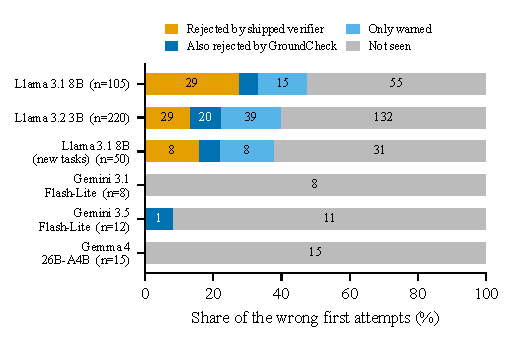
\includegraphics[width=\columnwidth]{figures/fig_e5_taxonomy}
\caption{What verification sees among the formulas each model gets wrong at attempt 1 (final system). Numbers are formulas.}
\label{fig:e5-taxonomy}
\end{figure}

\paragraph{Repair}
\begin{table*}[!t]
\caption{End-to-end execution accuracy (\%) of the production formula agent after up to two repair attempts, by repair strategy, with retrieved context. $\Delta$: percentage points over attempt 1; $p_{\text{Holm}}$: exact McNemar test against plain resampling (same tasks, paired), Holm-adjusted over the four feedback strategies of each model. Models whose first attempts are almost never rejected are omitted: no strategy has anything to repair.}
\label{tab:e5-repair}

\centering\footnotesize
\begin{tabular}{l rrr rrr rrr}
\toprule
& \multicolumn{3}{c}{\textbf{Llama~3.1 8B} (n=360)} & \multicolumn{3}{c}{\textbf{Llama~3.2 3B} (n=360)} & \multicolumn{3}{c}{\textbf{Llama~3.1 8B, new tasks} (n=180)} \\
\cmidrule(lr){2-4}\cmidrule(lr){5-7}\cmidrule(lr){8-10}
\textbf{Condition} & Acc. & $\Delta$ & $p_{\text{Holm}}$ & Acc. & $\Delta$ & $p_{\text{Holm}}$ & Acc. & $\Delta$ & $p_{\text{Holm}}$ \\
\midrule
Attempt 1 (no repair) & 70.8 & -- & -- & 38.9 & -- & -- & 72.2 & -- & -- \\
Resample (no feedback) & 71.1 & +0.3 & -- & 39.2 & +0.3 & -- & 72.8 & +0.6 & -- \\
Generic feedback & 72.2 & +1.4 & .125 & 39.7 & +0.8 & 1.000 & 72.8 & +0.6 & 1.000 \\
Shipped-verifier feedback & 74.2 & +3.3 & .007 & 39.7 & +0.8 & 1.000 & 74.4 & +2.2 & .750 \\
GroundCheck feedback & \textbf{74.4} & +3.6 & .001 & \textbf{40.0} & +1.1 & 1.000 & \textbf{75.0} & +2.8 & .375 \\
GroundCheck + suspicious & \textbf{75.3} & +4.4 & <.001 & \textbf{40.0} & +1.1 & 1.000 & \textbf{76.1} & +3.9 & .125 \\
\bottomrule
\end{tabular}
\end{table*}

Table~\ref{tab:e5-repair} and Figure~\ref{fig:e5} compare feedback strategies from the same first attempt. Asking again without feedback repairs almost nothing (\efASresample\%, $+$\efASresampleD{} points); a generic ``try again'' message gives \efASgeneric\% ($+$\efASgenericD{}); diagnostics from the shipped verifier \efASvonefb\% ($+$\efASvonefbD{}); and \gc{} diagnostics \efASvtwofb\% ($+$\efASvtwofbD{} points, 95\% interval [\efASvtwofbLo, \efASvtwofbHi]; \efASvtwofbFixed{} tasks fixed, none broken), better than resampling (Holm-adjusted $p$ \hmAHolmVtwoRes) and than the generic message ($p$ \hmAHolmVtwoGen). Also repairing on suspicious findings reaches \efASvtwofbplussusp\% ($+$\efASvtwofbplussuspD{}). The feedback of the two verifiers is not distinguishable here ($p$ \hmAHolmVtwoVone; they fix \efASvtwofbFixed{} and \efASvonefbFixed{} tasks), for the reason given above. The ordering is the same with the shipped chunk format (Table~\ref{tab:e5-repair-shipped}). Repair costs about \efAExtravtwofb{} extra model calls per task. The hosted models are absent from Table~\ref{tab:e5-repair} because they rarely give the verifier anything to reject.

\begin{figure}[t]
\centering
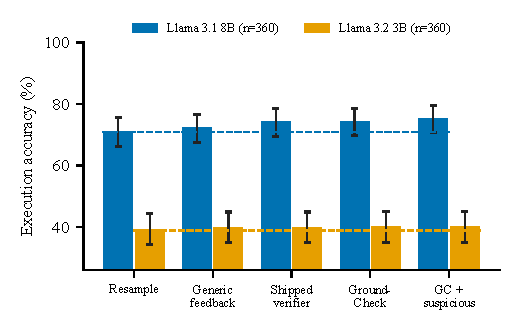
\includegraphics[width=\columnwidth]{figures/fig_e5_repair}
\caption{Execution accuracy after repair (GC: \gc) for the models whose attempts the verifier rejects often enough to compare strategies. Dashed lines: accuracy at attempt 1; error bars: 95\% Wilson intervals.}
\label{fig:e5}
\end{figure}

\paragraph{Run-to-run variation}
\ifdefined\sdASeeds
One sampled trajectory per task could mislead, so we reran the local models on the same tasks with \sdASeeds{} sampling seeds (Table~\ref{tab:e5-seeds}). Accuracy at attempt 1 with retrieved context is \sdARetr\% (SD \sdARetrSD{} points) for \efAName{} and \sdBRetr\% (SD \sdBRetrSD) for \efBName: the seed moves a model's accuracy by about a point, less than the differences between context formats or repair strategies that we interpret. For \efAName{} \gc{} feedback beats plain resampling in \sdASeedsBeat{} of \sdASeeds{} seeds, by \sdADvtwofbresample{} points on average over seeds and tasks (task-clustered 95\% interval [\sdADvtwofbresampleLo, \sdADvtwofbresampleHi]); against the shipped verifier's feedback the difference is \sdADvtwofbvonefb{} points [\sdADvtwofbvonefbLo, \sdADvtwofbvonefbHi]. For \efBName{} \gc{} feedback also beats resampling in \sdBSeedsBeat{} of \sdBSeeds{} seeds, but by only \sdBDvtwofbresample{} points [\sdBDvtwofbresampleLo, \sdBDvtwofbresampleHi]: a small effect that a single run (Table~\ref{tab:e5-repair}) cannot resolve.

\begin{table}
\caption{Run-to-run variation on the 360 main-set tasks: the same tasks rerun with 3 independent sampling seeds. The interval for the repair effect is a paired bootstrap over tasks of each task's outcome averaged over seeds.}
\label{tab:e5-seeds}

\centering\footnotesize
\begin{adjustbox}{max width=\columnwidth}\begin{tabular}{l rr}
\toprule
\textbf{Accuracy, mean (SD) over seeds} & \textbf{\shortstack[r]{Llama~3.1\\8B}} & \textbf{\shortstack[r]{Llama~3.2\\3B}} \\
\midrule
Attempt 1, active sheet only & 72.2 (0.3) & 35.8 (1.5) \\
Attempt 1, retrieved context & 71.4 (0.6) & 39.4 (0.7) \\
Resample (no feedback) & 71.6 (0.4) & 39.7 (0.7) \\
Generic feedback & 73.1 (0.8) & 40.2 (0.6) \\
Shipped-verifier feedback & 74.8 (0.7) & 40.4 (0.9) \\
GroundCheck feedback & 75.6 (1.1) & 40.8 (1.0) \\
GroundCheck + suspicious & 76.2 (0.8) & 41.0 (1.1) \\
\midrule
\gc{} feedback $-$ resample, points [95\% CI] & 4.0 [2.2, 5.9] & 1.1 [0.3, 2.2] \\
\gc{} feedback $-$ shipped feedback, points [95\% CI] & 0.7 [0.1, 1.6] & 0.5 [0.1, 1.0] \\
Seeds in which \gc{} beats resampling & 3 of 3 & 3 of 3 \\
\bottomrule
\end{tabular}\end{adjustbox}
\end{table}

\else
Further sampling seeds were not run for this version.
\fi

\paragraph{Does repair make failures safer?}
Accuracy counts whether the final cell is right and says nothing about what the wrong cells look like. Table~\ref{tab:e5-harm} accounts for every task under three policies. With \efAName, writing the first attempt unchecked leaves \hmAAsIsLoud{} cells that show an error and \hmAAsIsSilent{} that show a plausible wrong value, out of \hmAN. Withholding what \gc{} rejects, without repair, holds back \hmABlockWithheld{} formulas, all of them wrong (\hmAFalseWithheld{} correct formulas withheld), and leaves the silent errors as they were. Repairing with \gc{} feedback (Figure~\ref{fig:e5-fate}) fixes \hmAUnsafeVtwoFixed{} of the \hmAUnsafeN{} rejected attempts, but of the others \hmAUnsafeVtwo{} end as plausible wrong values and \hmAUnsafeVtwoLoud{} still show an error: the \emph{unsafe-repair rate} is \hmAUnsafeVtwoRate\% (shipped feedback: \hmAUnsafeVoneRate\%; resampling: \hmAUnsafeResRate\%, because it rarely changes anything). As a result the silent errors \emph{rise}, from \hmAAsIsSilent{} to \hmARepVtwoSilent, while the visible errors fall from \hmAAsIsLoud{} to \hmARepVtwoLoud. The picture is the same for \efBName{} (silent \hmBAsIsSilent{} to \hmBRepVtwoSilent, unsafe-repair rate \hmBUnsafeVtwoRate\%) and on the held-out tasks (\hmCAsIsSilent{} to \hmCRepVtwoSilent). \ifdefined\sdASeeds It holds across seeds: the unsafe-repair rate of \efAName{} averages \sdAUnsafevtwofb\% over the \sdASeeds{} seeds, ranging from \sdAUnsafevtwofbMin\% to \sdAUnsafevtwofbMax\%.\fi

\begin{table}
\caption{What ends up in the cell, as \% of tasks, under three policies: write the first attempt unchecked; withhold what \gc{} rejects and write the rest (no repair); repair with \gc{} feedback. \emph{Right}: evaluates to the gold value. \emph{Error}: the cell shows an error value. \emph{Silent}: a plausible but wrong value (the failure a user cannot see). \emph{Held}: nothing is written.}
\label{tab:e5-harm}

\centering\footnotesize
\begin{adjustbox}{max width=\columnwidth}\begin{tabular}{l l rrrr}
\toprule
\textbf{Model} & \textbf{Policy} & \textbf{Right} & \textbf{Error} & \textbf{Silent} & \textbf{Held} \\
\midrule
\multirow{3}{*}{Llama~3.1 8B} & Write as is & 70.8 & 18.6 & 10.6 & -- \\
 & Block rejected & 70.8 & 8.9 & 10.6 & 9.7 \\
 & Repair (\gc) & 74.4 & 12.5 & \textbf{13.1} & -- \\
\midrule
\multirow{3}{*}{Llama~3.2 3B} & Write as is & 38.9 & 30.6 & 30.6 & -- \\
 & Block rejected & 38.9 & 16.9 & 30.6 & 13.6 \\
 & Repair (\gc) & 40.0 & 24.2 & \textbf{35.8} & -- \\
\midrule
\multirow{3}{*}{Llama~3.1 8B new tasks} & Write as is & 72.2 & 16.1 & 11.7 & -- \\
 & Block rejected & 72.2 & 10.0 & 11.7 & 6.1 \\
 & Repair (\gc) & 75.0 & 12.2 & \textbf{12.8} & -- \\
\bottomrule
\end{tabular}\end{adjustbox}
\end{table}


Verification-guided repair therefore raises accuracy by turning some visible failures into correct formulas and others into invisible ones: of the visible errors it removes, only part become right. Blocking and showing the diagnostics has no such side effect, and the case for repair rests on how much a user's attention is worth. Since the outcome of a repaired formula is a valid-looking value, we regard an execution check, or showing the computed value next to the request, as the natural next step. An execution check in a scratch cell would catch the cells that show an error (\hmAAsIsLoud{} before repair and \hmARepVtwoLoud{} after, for \efAName) but none of the silent ones, which only the computed value, read against the request, can expose.

\ifdefined\exASame
\emph{Adding an execution check.} The cells that still show an error after repair are loud faults the workbook-state checks did not see. We therefore added a second stage to the pipeline, verify, repair, \emph{execute}: after \gc{} accepts a formula, it is evaluated in the workbook (in the add-on, in a scratch cell) and an error is sent back to the model (Table~\ref{tab:e5-exec}; first attempts regenerated with the same seed reproduced the stored one for \exASame{} of \exATotal{} tasks of \efAName). Of the \exALoudAfter{} cells that still show an error after \gc{} repair, the execution check fixes \exALoudFixed{}, leaves \exALoudStill{} and turns \exALoudToSilent{} into plausible wrong values; overall \exAExecCorrect{} formulas are right against \exAVtwoCorrect{} with repair alone (+\exAGained{}/$-$\exALost{} tasks, $p$ \exAP), and silent errors go from \exAVtwoSilent{} to \exAExecSilent. For \efBName{} (\exBSame{} tasks) the check fixes \exBLoudFixed{} of the \exBLoudAfter{} cells that still show an error after repair and turns \exBLoudToSilent{} into plausible wrong values; silent errors go from \exBVtwoSilent{} to \exBExecSilent. The check removes some visible errors but no silent ones: it cannot see them, and repairing an error can again produce a plausible wrong value, so the number of silent errors does not fall.

\begin{table}
\caption{What ends up in the cell (\% of tasks) when repair is followed by an execution check: after the verifier accepts a formula, the cell is evaluated and an error is sent back to the model. Only tasks whose regenerated first attempt reproduced the stored one are included, so all three policies cover the same tasks.}
\label{tab:e5-exec}

\centering\footnotesize
\begin{adjustbox}{max width=\columnwidth}\begin{tabular}{l l rrr}
\toprule
\textbf{Model} & \textbf{Policy} & \textbf{Right} & \textbf{Error} & \textbf{Silent} \\
\midrule
\multirow{3}{*}{Llama~3.1 8B} & Write as is & 75.2 & 16.2 & 8.6 \\
 & Repair (\gc) & 78.3 & 10.4 & 11.3 \\
 & Repair + execution & 80.1 & 7.6 & \textbf{12.2} \\
\midrule
\multirow{3}{*}{Llama~3.2 3B} & Write as is & 45.1 & 26.3 & 28.6 \\
 & Repair (\gc) & 46.5 & 19.2 & 34.3 \\
 & Repair + execution & 47.8 & 15.2 & \textbf{37.0} \\
\bottomrule
\end{tabular}\end{adjustbox}
\end{table}

\fi

\begin{figure}[t]
\centering
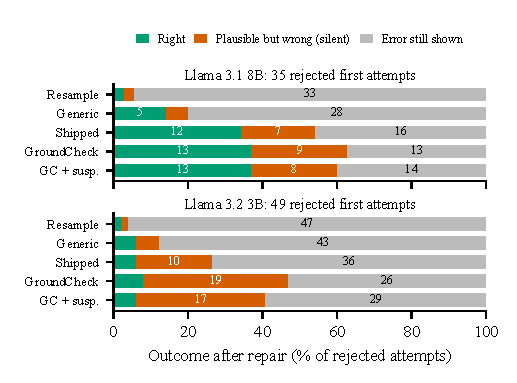
\includegraphics[width=\columnwidth]{figures/fig_e5_repair_fate}
\caption{Outcome of repair for the attempts \gc{} rejected, by strategy: right, a plausible but wrong value (silent), or an error still shown. Numbers are attempts; segments under 9\% are unlabelled.}
\label{fig:e5-fate}
\end{figure}

\paragraph{Where the models fail}
Accuracy by task template (Figure~\ref{fig:e5-templates}, Appendix~\ref{app:results}) shows the pattern behind the totals. The local models fail on the same few templates: \efATemplateZero{} of the \efNTemplates{} templates (the cross-sheet lookup) is solved on fewer than one task in twenty by \efAName{} and \efBTemplateZero{} by \efBName, whereas the hosted models' lowest template accuracies are \efDTemplateMin\%, \efETemplateMin\% and \efFTemplateMin\%. Requests that paraphrase the column names instead of quoting the headers are harder for the two local models on the main set (\efAFormS\% against \efAFormH\% for \efAName, \efBFormS\% against \efBFormH\% for \efBName) but not on the held-out set (\efCFormS\% against \efCFormH\%); we do not read more into it.
\ifdefined\efBN
\paragraph{A smaller model}
\efBName{} is correct at attempt 1 in \efBfinal\% of tasks (\efBflat\% with the active sheet only, $p$ \efBTestfinalvsflatP). It makes more of the errors that only \gc{} sees: the verifier rejects \efBCaughtTwo{} of its \efBWrong{} wrong first attempts, against \efBCaughtOne{} for the shipped one. But it makes little use of the feedback. In the main run repair raises accuracy by \efBSvtwofbD{} points ($p$ \efBSvtwofbP{} against attempt 1; \efBSvtwofbFixed{} tasks fixed), which no strategy distinguishes from resampling (Table~\ref{tab:e5-repair}); only the average over seeds resolves a gain of about a point. Feedback needs a model able to act on it. As an acceptance gate the verifier still separates the two groups: formulas it accepts are correct \efBGateAcc\% of the time and those it rejects \efBGateRej\%.
\fi
\paragraph{Hosted models}
The hosted models are right at attempt 1 on \efDfinal\%, \efEfinal\% and \efFfinal\% of their tasks (\efDflat\%, \efEflat\% and \efFflat\% with the active sheet only), so they leave the verifier almost nothing to do: they make few errors, most of them silent (\efDSilent{} of \efDWrong, \efESilent{} of \efEWrong, \efFSilent{} of \efFWrong), and no repair strategy has anything to repair. For models this accurate on these tasks the verifier is a safety net that costs nothing, and the benefit of the add-on comes from the context it supplies. This is no verdict on the value of verification for stronger models on harder work: \sheetfault{} tasks are single formulas over one or two tables, while workflow-level benchmarks find frontier agents failing far more often~\cite{zhu2026spreadsheetbench2}. The two Gemini runs were capped by the free tier's daily quota, so each covers the first tasks of a fixed hash order (\efDN{} and \efEN{} of the 360), a subset chosen without regard to difficulty; the Gemma run covers \efFN{}.


\ifdefined\sixN
\subsection{Why not ask the model?}
\label{sec:e6}
\begin{table}
\caption{A language-model critic (same model and context as the generator) versus the deterministic verifier on a stratified sample of \sheetfault{}; recall in \% when blocking only on rejection.}
\label{tab:e6}

\centering\footnotesize
\begin{adjustbox}{max width=\columnwidth}\begin{tabular}{l r rrr}
\toprule
\textbf{Fault group} & n & Critic & \gc & Either \\
\midrule
Structural & 25 & 44 & 100 & 100 \\
Symbols & 37 & 65 & 92 & 92 \\
Shape & 15 & 87 & 100 & 100 \\
Grounding & 14 & 29 & 0 & 29 \\
Circularity & 33 & 61 & 100 & 100 \\
Semantic & 16 & 38 & 19 & 38 \\
\midrule
All faults & 140 & 55.7 & 78.6 & 83.6 \\
Clean formulas rejected (FPR) & 161 & 21.1 & 0.0 & 21.1 \\
\bottomrule
\end{tabular}\end{adjustbox}
\end{table}

A critic given the same model and context (\sixN{} sampled instances, \sixFaults{} faulty; Table~\ref{tab:e6}) rejects \sixCriticR\% of faults and \sixCriticFPR\% of clean formulas (F1 \sixCriticF), against \sixVerR\% and \sixVerFPR\% for the verifier on the same sample (F1 \sixVerF). It catches only \sixCriticStructural\% of the structural faults, which a parser sees at no cost, and \sixCriticCircular\% of circular references (verifier: \sixVerCircular\%). It does catch \sixCriticOnlyCaught{} faults the verifier does not (chiefly \sixCriticOnlyWhere), against \sixVerOnlyCaught{} the other way round (the verifier flags the grounding cases but by policy does not reject them); combining the two raises recall to \sixEitherR\% but false positives to \sixEitherFPR\%. Asking the model is a poor replacement for a parser and at best a complement where the workbook cannot adjudicate.
\fi

\subsection{Context retrieval under a token budget}
\label{sec:e2}
When the whole workbook fits the budget, retrieval is moot: at \eTwoZeroFull{} tokens (10 tables) every ranking method, even random, retrieves all gold tables at a 1{,}500-token budget (\eTwoZeroComplete\% for the ranker). It becomes informative as workbooks grow. At \eTwoTables{} tables (\eTwoFull{} tokens, \eTwoReq{} requests, budget 1{,}500, \eTwoReduction\% fewer tokens than sending everything) the ranker keeps all gold tables in \eTwoRankerComplete\% of requests against \eTwoBmComplete\% for BM25 and \eTwoRandComplete\% for random, and the shipped agent's active-sheet context holds none (Table~\ref{tab:e2} and Figure~\ref{fig:e2}, Appendix~\ref{app:results}); at a 500-token budget the figures are \eTwoRankerCompleteSmall\% and \eTwoBmCompleteSmall\%. Adding column letters made every chunk longer, so the same budget holds fewer tables: the cost of the fix in Section~\ref{sec:e5}. Figure~\ref{fig:e2-scale} shows the same budget as the workbook grows: the ranker and BM25 are equal while everything fits, the gap opens as the workbook outgrows the budget, and the active-sheet context never holds the gold tables.

\begin{figure}[t]
\centering
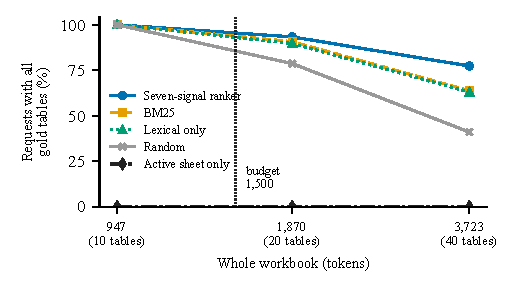
\includegraphics[width=\columnwidth]{figures/fig_e2_scale}
\caption{Share of requests whose prompt contains every gold table at a 1{,}500-token budget, as the workbook grows (10, 20 and 40 tables).}
\label{fig:e2-scale}
\end{figure}

\begin{table}
\caption{Gold-complete rate (\%) by request type at 40 tables, budget 1500. A: aggregate; B: lookup; C: ``change \emph{this} formula\textquotedblright{}. H: names the column; S: paraphrase only.}
\label{tab:e2-type}

\centering\footnotesize
\begin{adjustbox}{max width=\columnwidth}\begin{tabular}{l rrrrr}
\toprule
\textbf{Method} & A-H & A-S & B-H & B-S & C \\
\midrule
Ranker & 100 & 30 & 100 & 57 & 100 \\
Lexical only & 100 & 30 & 100 & 57 & 28 \\
Graph signals only & 28 & 28 & 50 & 50 & 100 \\
Ranker $-$ graph & 100 & 30 & 100 & 57 & 10 \\
BM25 & 100 & 33 & 100 & 57 & 28 \\
Random & 28 & 45 & 47 & 48 & 37 \\
\bottomrule
\end{tabular}\end{adjustbox}
\end{table}

Lexical overlap solves requests that name the data and graph signals those that do not (Table~\ref{tab:e2-type}): for ``change this to an average'' the ranker finds the table in \eTwoRankerC\% of requests, BM25 in \eTwoBmC\%, and the ranker without its two graph signals in \eTwoNoGraphC\%. The graph signals are redundant with each other, so removing one changes nothing. The structural signals add nothing on this benchmark. Paraphrase is the weak spot: with no shared word, \eTwoRankerAS\% (aggregates) and \eTwoRankerBS\% (lookups) of requests are gold-complete.

\subsection{Cost, and the fetch boundary (secondary)}
\label{sec:e3}
Analysis costs about 11 \code{SpreadsheetApp} calls plus \eScaleCallsPerSheet{} per sheet, independent of rows; verifying one formula costs \eScaleVerifyVone{} calls in the shipped verifier and \eScaleVerifyVtwo{} in \gc{} (a constant increase for column profiles, plus \eScaleVerifyPerSheet{} per sheet); CPU time stays below \eScaleMaxAnalyzeMs{} ms for analysis and \eScaleMaxVerifyMs{} ms for verification even at 2{,}000 formulas (Table~\ref{tab:e3} and Figure~\ref{fig:e3-cost}, Appendix~\ref{app:results}; Apps Script latency itself is not measured), negligible next to a model call.

The URL validator is a secondary result, included because the same check-before-acting idea guards the add-on's one outbound channel. On the corpus of Table~\ref{tab:ssrf} (Appendix~\ref{app:results}), the shipped URL filter blocks \ssrfvoneRecall\% of \ssrfBlock{} must-block URLs (\ssrfvoneBypass{} bypasses, including every decimal, hexadecimal and octal encoding of loopback and private addresses, \code{127.1}, and every internal-only name) and wrongly blocks \ssrfvoneFalseBlock\% of \ssrfAllow{} benign URLs, because it matches substrings of the whole URL (\code{https://210.1.2.3/} is rejected for containing \code{10.1.2.3}). The parse-and-classify validator blocks \ssrfvtwoRecall\% (95\% interval lower bound \ssrfvtwoCILo\%) with \ssrfvtwoFalseBlock\% false blocks. The corpus was built by us from known bypass classes, so it measures coverage, not adversarial robustness; one bypass (a backslash before \code{@}) was found by the first run and fixed.
